\chapter{Materials and methods}\label{cap:materials}

This chapter describes in detail used datasets, processing techniques and the methods used, and comments on the reasoning behind the choices.
Hopefully, by the end of this chapter the reader will be confident in their ability to recreate the framework from scratch.
The code of the project on my GitHub might be a helpful addition for that.

\section{Lysva field inventory dataset}

The main original dataset used in the study is the Lysva field inventory dataset, named by the closest town to its location.
The dataset is released into open access with an accompanying paper that describes the data in detail and provides a basic baseline for individual tree detection \cite{dubrovinExplorationPropertiesPoint2024}.
The study area is located in Perm Krai, Russia, 86 kilometers to the east of Perm.
The dataset consists of a field inventory of 3600 trees across 10 rectangular ground plots 100 meters in lengths and 50 meters in width fully covered by a UAV LiDAR and RGB orthophoto surveys.
Figure~\ref{fig-lysva-roi} shows the locations of the ground plots over the full size RGB orthophoto and a visualization of the field inventory for a single plot on top of the LiDAR point cloud.
Colored points represent trees, with different colors mapping to different species.
The point cloud is visualized as a 2D scatter plot with points colored by height (darker points are lower, brighter points are higher).

\begin{figure}
\centering{
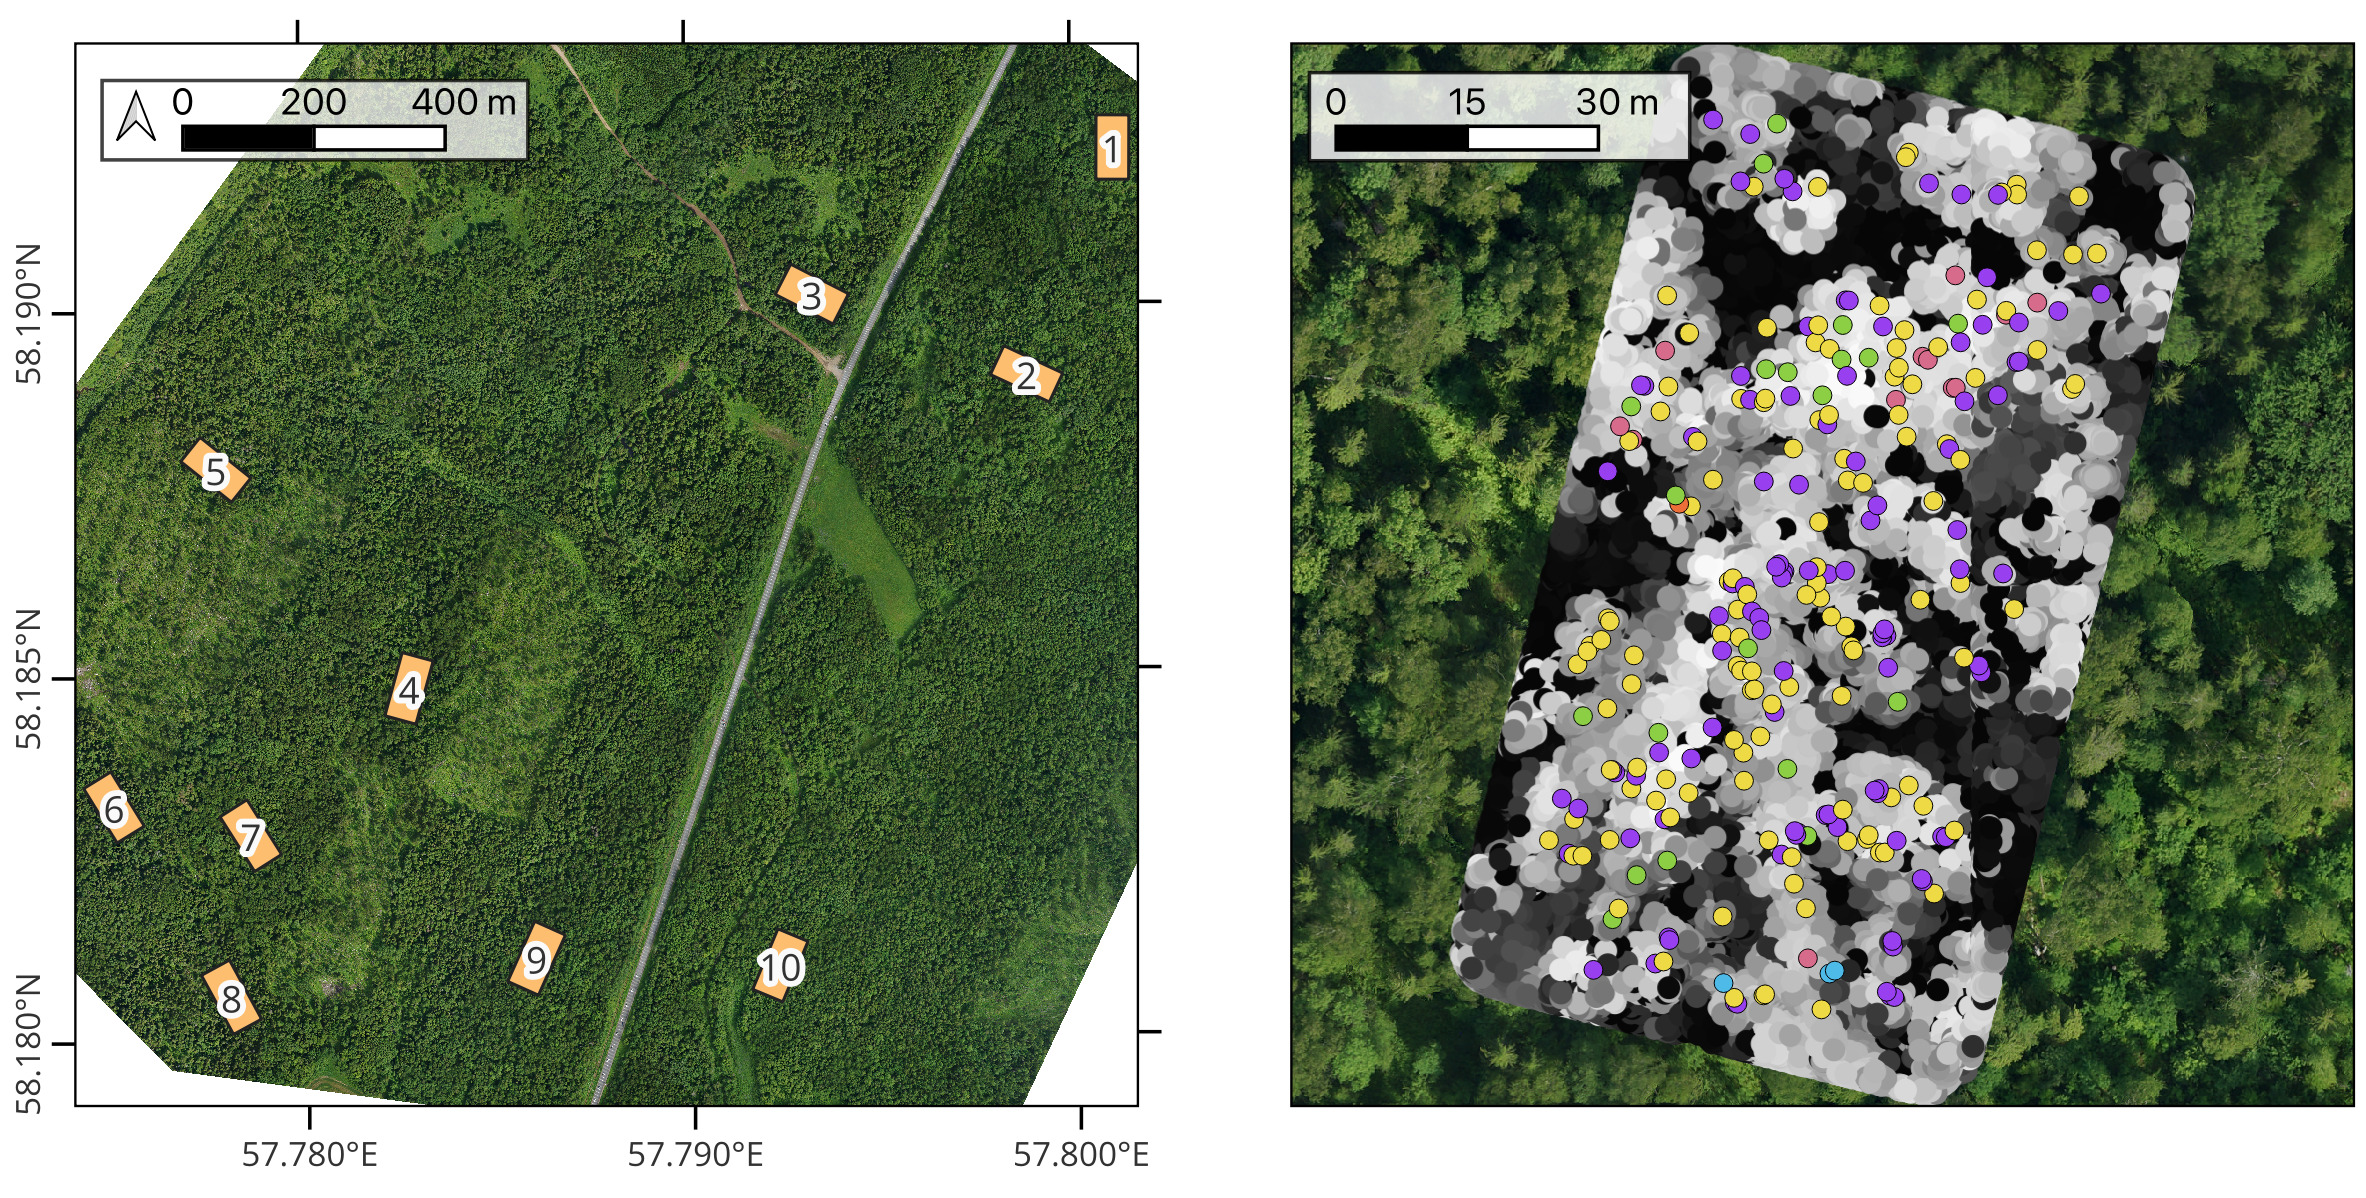
\includegraphics[width=\textwidth]{../images/lysva_roi.jpg}
}
\caption{\label{fig-lysva-roi}The study region for the Lysva field
inventory dataset. \textbf{Left}: The locations of field survey plot
boundaries on a full-size RGB orthophoto. Each plot is a 50 by 100 meter
rectangle, with every tree within measured and recorded. Buffered
cutouts of the orthophoto come with the dataset, along with LiDAR point
clouds. \textbf{Right}: A close up of plot number 4. Each colored point
represents a single tree of a different species, on top of a point cloud
colored by the value of the height of each point (lower points are dark,
higher points are bright) and the same orthophoto. Figure reused from
(Dubrovin and Fortin 2024).}
\end{figure}


The field inventory is a tabular dataset where every row represents a single tree.
Table~\ref{tbl-inventory-example} shows a random sample of entries from the field inventory table.
Every tree is represented by a point in UTM 40N coordinate reference system (EPSG:32640).
Every tree has a species label and diameter at breast height (dbh), measured with calipers at 1.3 m from the ground at two perpendicular directions and averaged.
Figure~\ref{fig-lysva-species-distribution} shows the distribution of species in the data: the dominant species is spruce, but overall the trees are evenly split between deciduous and coniferous, 1793 and 1807 respectively, with seven species in total: spruce, birch, fir, aspen, tilia, alder, and willow.
Approximately 20\% of the trees have height data measured during the inventory, and 10\% have ages measured on core samples, shown in the table in meters and years respectively.

\begin{longtable}[]{@{}lllllllllll@{}}

\caption{\label{tbl-inventory-example}Example of data in the field
inventory table. Each row is a recorded tree.}

\tabularnewline

\toprule\noalign{}
plot & tree\_no & species & d1 & d2 & dbh & age & height & angle &
comment & geometry \\
\midrule\noalign{}
\endhead
\bottomrule\noalign{}
\endlastfoot
7.0 & 111.0 & Birch & 23.0 & 23.0 & 23.00 & NaN & NaN & 0.0 & None &
POINT (545784.419 6449359.132) \\
5.0 & 136.0 & Fir & 23.5 & 23.0 & 23.25 & 90.0 & 17.5 & 0.0 & Rotten &
POINT (545721.242 6449901.051) \\
3.0 & 119.0 & Aspen & 36.1 & 42.1 & 39.10 & 89.0 & 25.5 & 0.0 & None &
POINT (546630.326 6450158.241) \\
9.0 & 345.0 & Spruce & 19.7 & 22.0 & 20.85 & NaN & 15.9 & 0.0 & None &
POINT (546201.645 6449118.199) \\
6.0 & 267.0 & Spruce & 12.9 & 12.9 & 12.90 & NaN & NaN & 0.0 & None &
POINT (545568.842 6449407.13) \\

\end{longtable}

\begin{figure}
\centering{
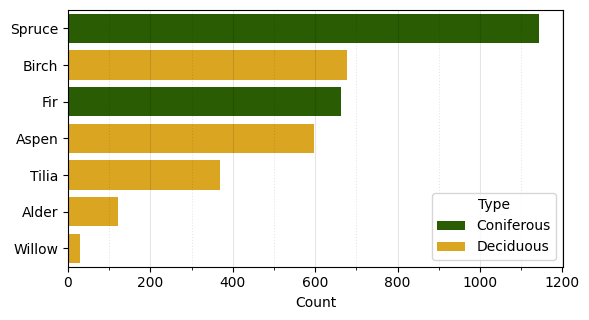
\includegraphics[width=\textwidth]{../images/03a_lysva_dataset-fig-lysva-species-distribution-output-1.png}
}
\caption{\label{fig-lysva-species-distribution}Distribution of species
in the Lysva field inventory dataset. The dominant species is spruce,
but overall the split between coniferous and decidious species is even:
there are 1807 coniferous and 1793 deciduous trees. Figure reused from
(Dubrovin and Fortin 2024).}
\end{figure}

The LiDAR sensor used for the survey is AGM-MS3 produced by AGM Systems.
It has 640 kHz acquisition rate, 300-meter range, and spatial accuracy of 3–5 centimeters.
The raw point clouds were processed with the combination of the AGM ScanWorks software from the sensor vendor and the TerraScan software.
The point clouds were preprocessed by removing duplicate points and high and low noise points.
The duplicate removal was run with a threshold distance between points of 1 mm.
Noise was removed by visually inspecting the point cloud and manually selecting height thresholds to cut off points that are lower than the ground or higher than the canopies.
Ground point classification was performed and ground points were used to normalize height by subtracting the ground level from the Z coordinate of every point.
Height normalization allows treating the Z coordinate as height above ground rather than the absolute elevation, which simplifies many subsequent steps.
The camera used for the orthophoto survey is Sony A6000.
The resolution of the orthophoto is 7 cm per pixel.
Figure~\ref{fig-example-3d-point-cloud} is a 3D visualization of the point cloud over plot number 10.
It shows the unmodified point cloud on the left, with points colored by height above ground, and a point cloud enriched with color information by sampling the orthophoto at the planar coordinates of the points.
Figure~\ref{fig-example-ortho} shows the orthophoto for the same plot.
The carrier UAV was configured to follow the terrain at 150 meter height using the SRTM elevation map as a reference \cite{farrShuttleRadarTopography2000}.

\begin{figure}
\begin{minipage}{0.50\linewidth}
\centering{
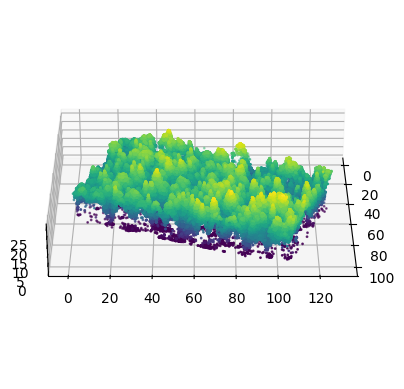
\includegraphics[width=\textwidth]{../images/03a_lysva_dataset-fig-example-3d-point-cloud-output-1.png}
}
\subcaption{\label{fig-example-3d-point-cloud-1}Points colored by
height.}
\end{minipage}
\begin{minipage}{0.50\linewidth}
\centering{
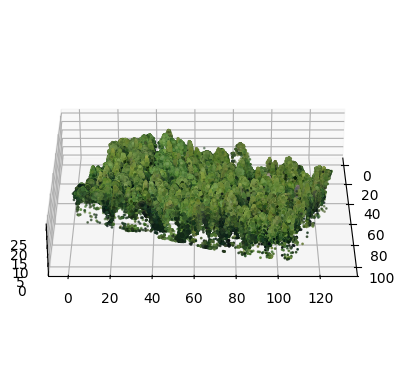
\includegraphics[width=\textwidth]{../images/03a_lysva_dataset-fig-example-3d-point-cloud-output-2.png}
}
\subcaption{\label{fig-example-3d-point-cloud-2}Points assigned color by
sampling the orthophoto.}
\end{minipage}
\caption{\label{fig-example-3d-point-cloud}A 3D visualisation of the UAV
LiDAR point cloud of plot 10.}
\end{figure}

\begin{figure}
\centering{
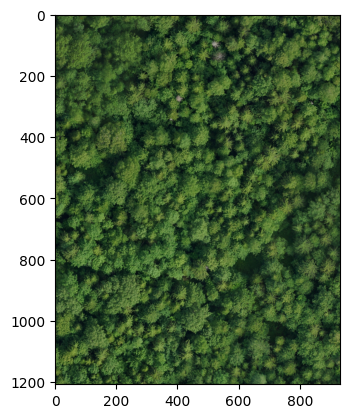
\includegraphics[width=\textwidth]{../images/03a_lysva_dataset-fig-example-ortho-output-1.png}
}
\caption{\label{fig-example-ortho}A visualisation of the orthophoto of
plot 10.}
\end{figure}

Table~\ref{tbl-lysva-plot-stats} shows some descriptive statistics for each plot in the field inventory: the number of trees in the plot, average LiDAR point density in points per square meter, and dominant species type.
The overall average point density is 37 points per square meters.
Exactly half of the plots are predominantly coniferous and half are predominantly deciduous.
Figure~\ref{fig-lysva-canopy-structure} shows two of point clouds clipped by plot bounds in 3D, highlighting the differences in canopy structure complexity between predominantly deciduous and coniferous plots.
The figure highlights that the forest is indeed dense and mixed, with non-uniform, complex canopy structure.

\begin{longtable}[]{@{}llll@{}}

\caption{\label{tbl-lysva-plot-stats}Statistics for the plots in the
Lysva dataset.}

\tabularnewline

\toprule\noalign{}
Plot & Tree count & Point density & Dominant type \\
\midrule\noalign{}
\endhead
\bottomrule\noalign{}
\endlastfoot
1.0 & 420 & 31.7 & Deciduous \\
2.0 & 365 & 47.9 & Deciduous \\
3.0 & 332 & 40.3 & Deciduous \\
4.0 & 261 & 33.5 & Coniferous \\
5.0 & 208 & 14.2 & Coniferous \\
6.0 & 290 & 39.1 & Coniferous \\
7.0 & 408 & 41.9 & Deciduous \\
8.0 & 341 & 35.5 & Coniferous \\
9.0 & 459 & 42.1 & Coniferous \\
10.0 & 518 & 42.9 & Deciduous \\

\end{longtable}

\begin{figure}
\centering{
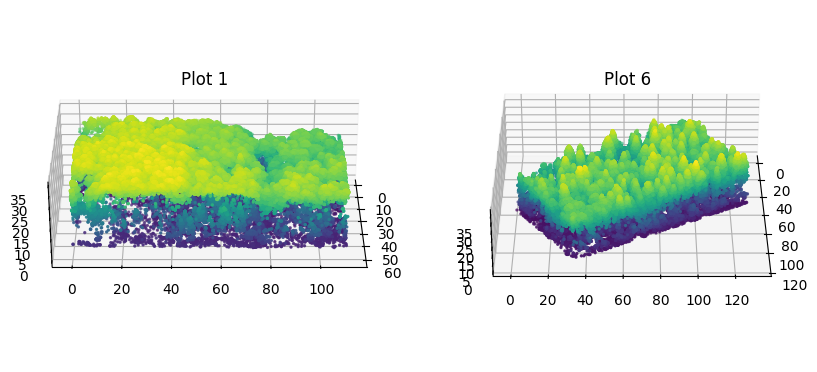
\includegraphics[width=\textwidth]{../images/03a_lysva_dataset-fig-lysva-canopy-structure-output-1.png}
}
\caption{\label{fig-lysva-canopy-structure}3D visualizations of point
clouds from plot 1 (predominantly deciduous) and plot 6 (predominantly
coniferous). Note the difference in the canopy structure: it is
relatively easy to tell confifiers apart visually, while deciduous
species do not have pronounced shapes and are hard to discriminate.
Figure reused from (Dubrovin and Fortin 2024).}
\end{figure}

\subsubsection{On using intensity-based features}\label{sec-intensity-based-features}

Even though some sources report intensity-based features as some of the most important ones \cite{shiImportantLiDARMetrics2018}, the features seem to me unreliable in the context of forestry because of the physics of light reflection.
There are simply too many factors that affect the amplitude of the reflected signal, which might be useful when imaging stable targets such as urban environments but become completely unpredictable on highly unstable targets such as trees: they move in the wind in the time span of a single survey, they grow in the time span between repeated surveys, the leaves and branches are angled in every possible way.
Moreover, the quality of the recorded intensities highly depends on the used sensor.
As an example, Figure~\ref{fig-intensity-with-example} shows the distribution of intensity values for every point in the Lysva dataset, and shows plot number 10 in 3D with points colored by their recorded intensity.
The distribution of intensities seems like an artifact of faulty quantization (the fact that the maximum overall value is 63 makes me suspect it is stored by the hardware using a 6-bit unsigned integer, probably an ad hoc optimization by the sensor vendor).
With this distribution in mind, it is not surprising that coloring points by their intensity values results in images that look like noise, and there is no signal to be exploited for predictive modeling.

\begin{figure}
\begin{minipage}{0.50\linewidth}
\centering{
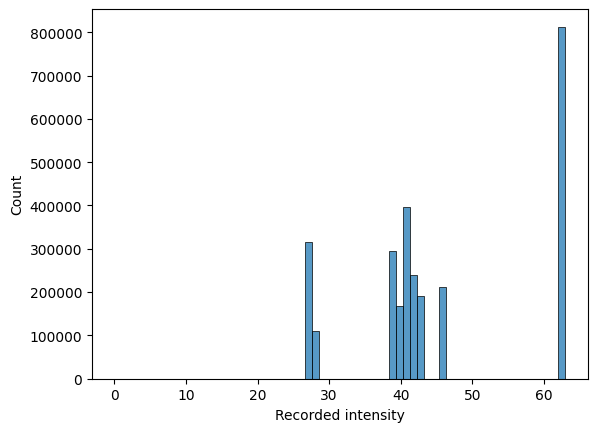
\includegraphics[width=\textwidth]{../images/03a_lysva_dataset-fig-intensity-with-example-output-1.png}
}
\subcaption{\label{fig-intensity-with-example-1}Distribution of
intensity over all points in the Lysva dataset.}
\end{minipage}
\begin{minipage}{0.50\linewidth}
\centering{
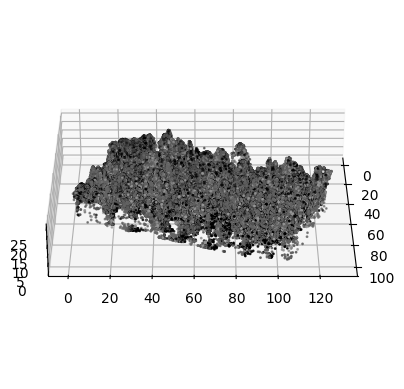
\includegraphics[width=\textwidth]{../images/03a_lysva_dataset-fig-intensity-with-example-output-2.png}
}
\subcaption{\label{fig-intensity-with-example-2}A point cloud of plot 10
with points colored by intensity.}
\end{minipage}
\caption{\label{fig-intensity-with-example}An example of the
unreliability of the intensity attribute.}
\end{figure}

Some sensors do provide more consistent values.
However, relying on intensity-based features limits the applicability of developed models and methods, as any such model would surely fail on data like this.

\subsubsection{Comparison to other datasets}

Our dataset is in many ways similar to the NewFor benchmark \cite{eysnAlpineITDBenchmark2015}.
It serves the same purpose and also offers overlapping field survey ground plots and UAV LiDAR point clouds.
There are, however, many notable differences.
The NewFor benchmark covers much more diverse regions, including ground plots from France, Italy, Switzerland, Austria, and Slovenia, while all our data comes from the same area.
The tree species covered by the datasets are also different: both contain spruce and fir, but the NewFor data also has beech, Scots pine, larch, sycamore, and poplar, while ours also has birch, aspen, tilia, alder, and willow.
Our dataset has more than twice as many individual trees as the Alpine benchmark, and the forest is denser and more complex, making it more complicated to detect trees in.
Our data contains very mild terrain variations, while the slopes of the terrain in Alpine data are very steep, which plays a role during height normalization, since subtraction of steep terrain introduces artificial slope to the points in the canopy, changing the overall shape of the tree.
Our dataset has an additional information source – an RGB orthophoto that allows development of algorithms that fuse multimodal data, which, we believe, is a key to success in such complex environments.
Our dataset has species labels for every surveyed tree, but only partial coverage of tree heights and no timber volume information at all.

Another similar dataset is the NeonTreeEvaluation Benchmark \cite{weinsteinDataNeonTreeEvaluationBenchmark2022}, which offers bounding box annotation for tree detection across a wide range of different forest types.
It offers coregistered RGB, LiDAR, and hyperspectral images over 31,000 individual trees.
The main difference in the reference data between the NeonTreeEvaluation Benchmark and our dataset is the source: our data comes from a field inventory and thus has additional tree information that can be used in downstream tasks, such as species classification or timber volume prediction, while the NeonTreeEvaluation Benchmark annotations are created from the RGB photo and thus only offer the positions and sized of trees.

Another dataset is the IDTReeS 2020 Competition Data \cite{gravesIDTReeS2020Competition2020} aimed to develop algorithms for delineation and species classification of individual tree crowns in RGB, LiDAR, and hyperspectral data.
It offers bounding box annotations for 1200 individual trees covered by RGB, LiDAR, and hyperspectral images in 3 national forests in the USA.
Similarly, the source of the data is annotation of images, not a field inventory.

There are also datasets available that don't have LiDAR point cloud coverage, or use terrestrial LiDAR instead of UAV LiDAR, or use photogrammetric point clouds instead of LiDAR  point clouds.
We do not mention them here because we specifically focus on UAV LiDAR.

\section{Individual tree point clouds dataset}\label{sec-individual-trees-dataset}

The main dataset used for training the models is a collection of point clouds of individual trees, referred to in this text as tree clouds, extracted manually from larger UAV LiDAR point clouds.
The dataset is released into open access, and was originally presented in \cite{dubrovinExplorationPropertiesPoint2024}, although it has been expanded since and now contains twice as many individual trees.
It consists of 394 trees, 192 of which are extracted from the previously described Lysva survey, and 202 from other surveys in Perm Krai.
The distinction between the parts is important because the Lysva dataset has RGB orthophoto coverage, making it possible to infuse the tree clouds with orthophoto-based features.
Thus, for training the tree segmentation networks that rely on these features, the effective size of the dataset is 192 tree clouds, as only the former part is used.
However, the whole dataset is used for training regression and classification models that process segmented trees.

Figure~\ref{fig-individual-trees-species-distribution} shows the distribution of species in the individual tree point clouds dataset.
The split between coniferous and deciduous trees is almost even: there are 202 coniferous and 193 deciduous trees.
There are seven species in total: spruce, birch, aspen, pine, fir, alder, and tilia, with most focus on 4 most important species listed first.
Note the presence of pine trees, which are not present in the Lysva field inventory data, and the absence of willow trees.
All the pine trees are from other field surveys.
Willows are skipped intentionally, since they are of little interest in terms of timber harvesting: they are considered low quality, and their ripening cycle is mismatched with main timber species – when the overall plot is ready to be harvested, the willows are already rotten.

\begin{figure}
\centering{
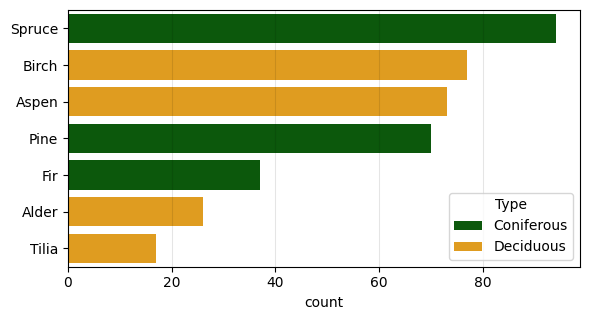
\includegraphics[width=\textwidth]{../images/03b_individual_trees-fig-individual-trees-species-distribution-output-1.png}
}
\caption{\label{fig-individual-trees-species-distribution}Distribution
of tree species in the individual trees dataset. It contains 394 point
clouds of individual trees: 201 coniferous and 193 deciduous. Note the
presence of pine trees, as there are no pine trees in the Lysva field
inventory -- all of the pines come from other field surveys.}
\end{figure}


Figure~\ref{fig-individual-trees-visualization} is a visualization of the data.
It shows a random tree of every species as a 2D scatter plot and a single spruce as a 3D scatter plot with points colored by height.
Because the observations are made from above, many trees have the highest concentrations of points at the top of their canopy and a very limited number of points along the trunk.
Additionally, slight slopes of the terrain manifest as artificial tilt in some of the trees because of the height normalization of the original point cloud.

\begin{figure}
\begin{minipage}{0.7\linewidth}
\centering{
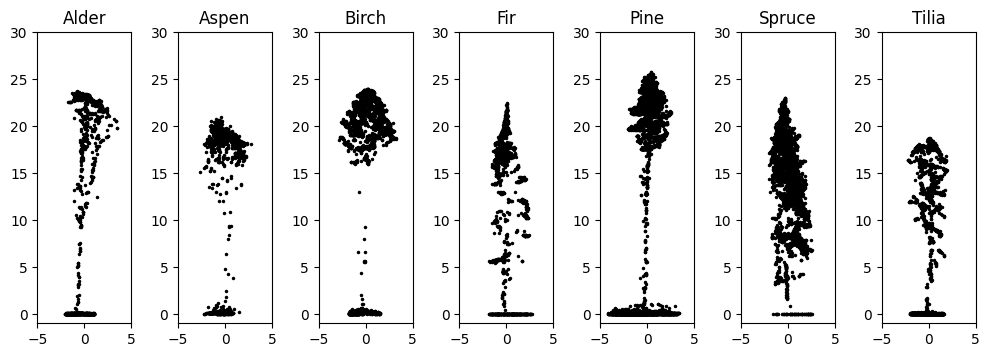
\includegraphics[width=\textwidth]{../images/03b_individual_trees-fig-individual-trees-visualization-output-1.png}
}
\subcaption{\label{fig-individual-trees-visualization-1}Cross-sections
of random trees of every species (ignoring the Y dimension).}
\end{minipage}
\begin{minipage}{0.29\linewidth}
\centering{
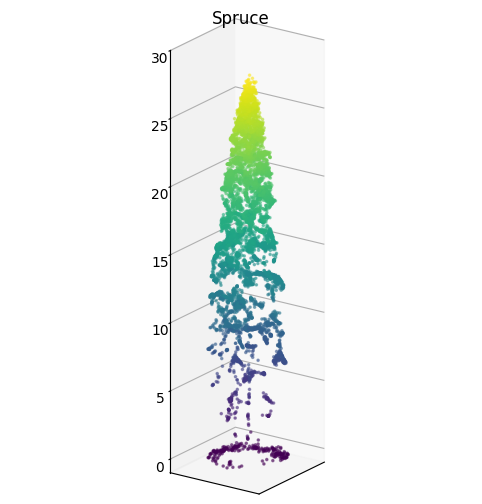
\includegraphics[width=\textwidth]{../images/03b_individual_trees-fig-individual-trees-visualization-output-2.png}
}
\subcaption{\label{fig-individual-trees-visualization-2}A spruce in 3D.}
\end{minipage}
\caption{\label{fig-individual-trees-visualization}Visualizations of the
individual tree point clouds in the dataset. Most of the tree clouds are
top-heavy because of the observation from above, and some are
artificially tilted because of slight terrain slopes and height
normalization. The ground points are present.}
\end{figure}

An important note is that the extracted trees were not chosen for extraction randomly but were selected by humans based on whether it was possible and relatively easy to separate from the surrounding trees.
So there is a selection bias in there favoring the trees that are easily separable, standing outside of large dense clusters.
Because of that the trees don't exactly represent what a tree closely surrounded by other trees is like in a point cloud.
It is especially apparent in very pronounced trunks of all the visualized trees.
In a dense forest, such as the one visualized in Figure~\ref{fig-lysva-canopy-structure}, there is hardly ever enough penetration for such detailed trunk coverage.
In fact, as mentioned in the literature review, good coverage of trunks is an immensely useful feature of terrestrial LiDAR surveys, which consistently show very good results using algorithm that segment trees from the trunk up.

\section{Synthetic forests generated from individual trees}\label{sec-synthetic-forest-dataset}

To train tree segmentation models, training data where every point is assigned to an individual tree is required. Data like that is very labor-intensive to label. An alternative way to create such data is by generating it from patches of forest with every point assigned to a tree is by combining point clouds of individual trees  into synthetc

A patch of fixed size, filled by randomly sampled trees and the ability to add overlap.

\begin{figure}
\begin{minipage}{0.50\linewidth}
\centering{
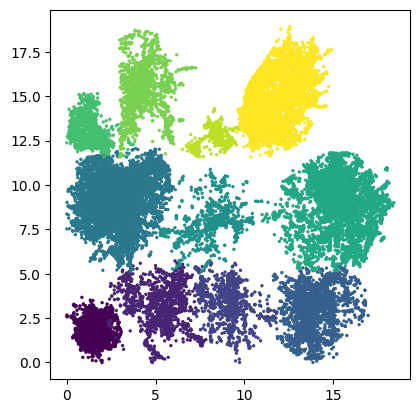
\includegraphics[width=\textwidth]{../images/03c_synthetic_forest-fig-synthetic-forest-patch-example-1-output-1.png}

}

\subcaption{\label{fig-synthetic-forest-patch-example-1-1}abc}

\end{minipage}%
%
\begin{minipage}{0.50\linewidth}

\centering{

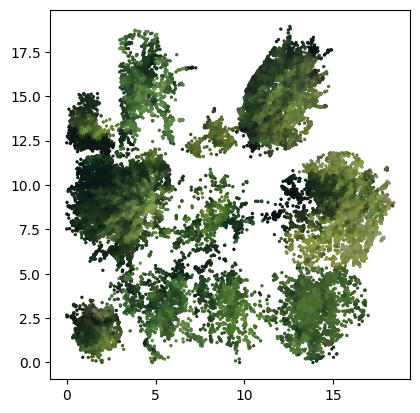
\includegraphics[width=\textwidth]{../images/03c_synthetic_forest-fig-synthetic-forest-patch-example-1-output-2.png}

}

\subcaption{\label{fig-synthetic-forest-patch-example-1-2}abc}

\end{minipage}%
\newline
\begin{minipage}{0.50\linewidth}

\centering{

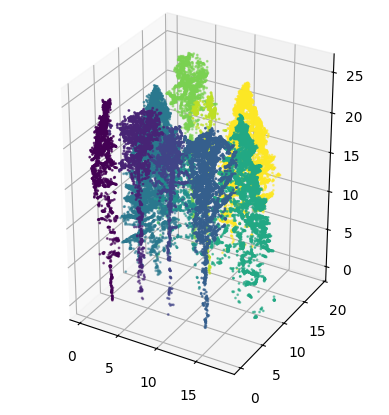
\includegraphics[width=\textwidth]{../images/03c_synthetic_forest-fig-synthetic-forest-patch-example-1-output-3.png}

}

\subcaption{\label{fig-synthetic-forest-patch-example-1-3}abc}

\end{minipage}%
%
\begin{minipage}{0.50\linewidth}

\centering{

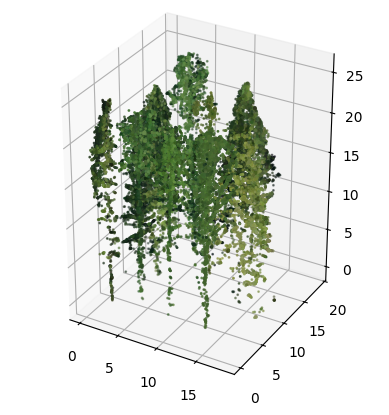
\includegraphics[width=\textwidth]{../images/03c_synthetic_forest-fig-synthetic-forest-patch-example-1-output-4.png}

}

\subcaption{\label{fig-synthetic-forest-patch-example-1-4}cde}

\end{minipage}%

\caption{\label{fig-synthetic-forest-patch-example-1}A 3D visualisation
of the UAV LiDAR point cloud of plot 10.}

\end{figure}

(show example patches of different size)
(show example patches colored by RGB and different false color combinations)

Each tree has features sampled from preprocessed orthophoto (multiscale basic features).

Fixed size is better than fixed number because of the scale normalization.

- Height threshold applied

\section{Training tree segmentation neural networks}

The architecture chosen to serve as the tree segmentation network is the PointNet++ \cite{qiPointNetPlusPlus2017}, described in detail in Section~\ref{sec-ml-dl}.
It is a relatively simple architecture, and further potential quality improvements might be achieved by using more modern and advanced architectures instead.
However, the main goal of this thesis was to develop and verify an overall framework, and thus the choice was set on a model that is simple to implement and work with to allow easy experimentation with other parts of the proposed system.

The architecture of the used PointNet++ is similar to the segmentation architecture shown in @fig-pointnet2-architecture.
The main differences are the use of one more stacked set abstraction layer to make the network deeper, and the use of a regression head that predicts a continuous value for each point instead of a classification head that predicts per-point class scores, since the model needs to assign a unique ID to every tree in the patch.
The three stacked set abstraction layers have the proportions of points sampled set to 0.75, 0.5, and 0.5, and neighborhood radii for feature aggregation set to 0.1, 0.2, and 0.4.
Note that the scale of the input is normalized (see next subsection for details), so the radii are not in meters.
The model has 30 million trainable parameters.

\subsection{Coordinate and feature normalization}

It's a well established practice to scale the inputs to neural networks that is known to improve the speed and accuracy of gradient descent convergence \cite{bishop2006pattern}.
Before going through the network, a set of augmentations and transformations is applied to each synthetic forest patch.
The augmentations are described in detail with visualized examples in @sec-augmentations.
The transformations include scale and feature normalization – the coordinates are centered and normalized to the interval $(-1, 1)$ and the features are normalized to sum up to 1.

\subsection{Data augmentation}\label{sec-augmentations}

The primary objective of data augmentation is to enhance the quantity, quality, and variety of data used for training \cite{mumuniDataAugmentationComprehensive2022}.
This is especially important when the sizes of the available datasets are limited, like in the case of the individual trees data that is the base of the synthetic forest datasets.

Carefully selected augmentations allow increasing the effective dataset size.
However, it is important to pay attention that the chosen augmentations keep the transformed examples semantically equivalent to the original.
A readily understandable example of a bad augmentation in the task of digit classification, which is often used as the "hello world" of deep learning with the MNIST dataset of handwritten digits \cite{deng2012mnist}, is a vertical flip, as most digits lose meaning when upside down.
A flip is also a bad augmentation example for a synthetic forest patch described in Section~\ref{sec-synthetic-forest-dataset}, as it changes the order of the trees within a patch, thus breaking the labels.

In the scenario when the data for is created by combining several smaller inputs, there is a possibility of applying augmentations on two different scales.
The most simple approach is to treat a synthetic forest patch as a whole and apply augmentations directly to it.
However, it is also possible to apply per-tree augmentations, effectively increasing the size of the underlying tree set from which synthetic forest patches constructed.
Both types of augmentations are used in training tree segmentation networks, described in detail in the following sections.

\subsubsection{Per-tree augmentations}

The first transformation that changes the shape but doesn't affect any semantics for an individual tree is a random rotation around the vertical axis.
A tree remains completely the same when rotated, but the coordinates of all points change.
Figure~\ref{fig-random-rotate-effect} shows the effect of applying random rotation transformation of different magnitudes to a single aspen tree.
For visualization purposes, the rotation is forced to apply with full magnitude for every parameter.
During training, the angle is uniformly sampled from the specified range.
For the final tree segmentation model, the range is set to $[-180, 180]$ degrees, as no amount of rotation breaks the semantics.

\begin{figure}
\centering{
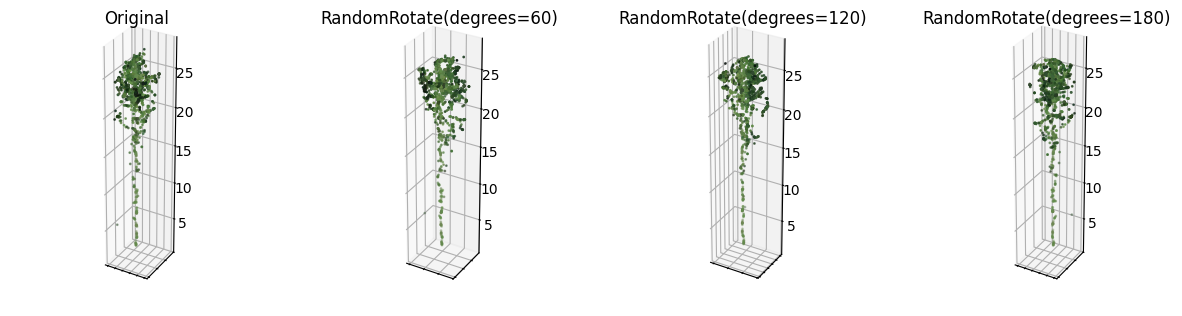
\includegraphics[width=\textwidth]{../images/03d_augmentations-fig-random-rotate-effect-output-1.png}
}
\caption{\label{fig-random-rotate-effect}Visualization of the random
rotation around Z axis augmentation on a single aspen tree. The effect
is forced to happen with full amplitude for visualization purposes,
during training a rotation angle is uniformly sampled from a set range.}
\end{figure}

Another transformation that keeps the tree the same but changes the coordinates of the points is random scaling.
It simply multiplies the coordinates by a scaling factor, making the tree larger or smaller in all directions.
Unlike random rotation around the vertical axis, however, the range needs to be chosen much more carefully, as there is a possibility of making unrealistically large or small trees that would confuse the model during training.
Figure~\ref{fig-random-scale-effect} shows the effect of applying random scale transformation to a single aspen tree.
Again, for purposes of visualization, the scale is forced to apply with full magnitude.
During training, the scale is uniformly sampled from the specified range.
For the final tree segmentation model, the range is set to $[0.8, 1.2]$.

\begin{figure}

\centering{
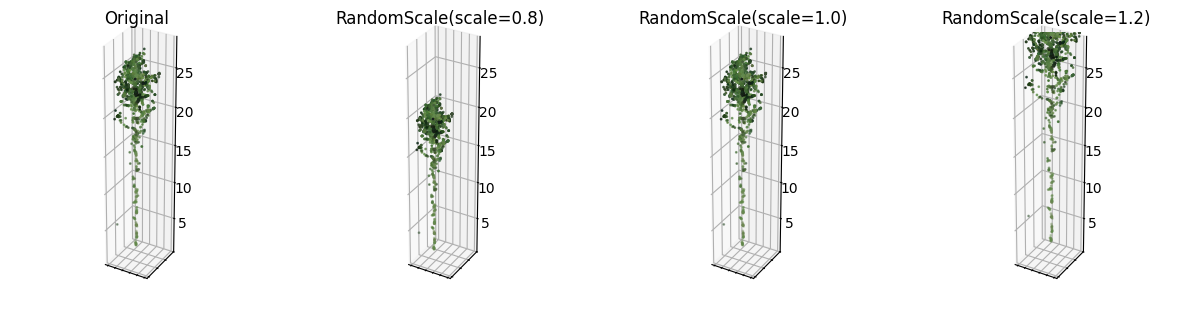
\includegraphics[width=\textwidth]{../images/03d_augmentations-fig-random-scale-effect-output-1.png}
}
\caption{\label{fig-random-scale-effect}Visualization of the random
scale augmentation on a single aspen tree. The effect is forced to
happen with full amplitude for visualization purposes, during training a
scale factor is uniformly sampled from a set range.}
\end{figure}

Note that the random jitter augmentation is applied before the scale normalization.
It matters because the augmentation's only parameter is the translation range, which depends on the scale.
The parameters on the figure are thus in meters.

\begin{figure}
\centering{
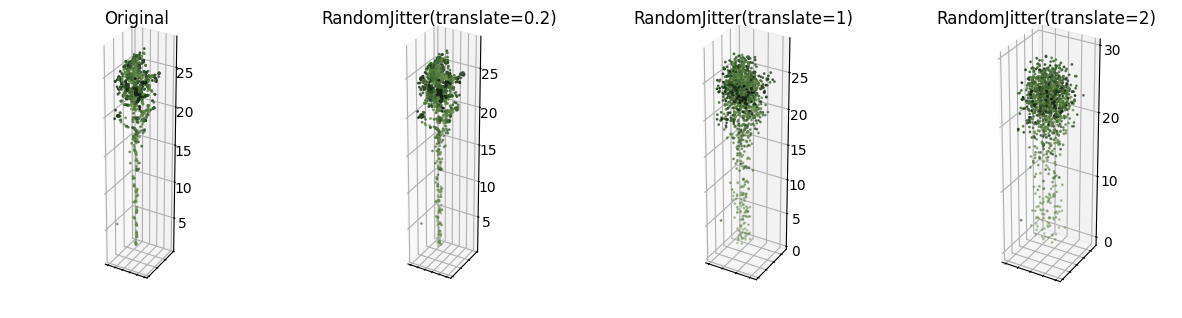
\includegraphics[width=\textwidth]{../images/03d_augmentations-fig-random-jitter-effect-output-1.png}
}
\caption{\label{fig-random-jitter-effect}Visualization of the random
jitter augmentation on a single aspen tree. The translation magnitude is
uniformly sampled from a set range for every point.}
\end{figure}

Another useful effect augmentations can provide is to make synthetic data look more like real data.
As was mentioned in Section~\ref{sec-individual-trees-dataset}, there is a selection bias in the dataset of individual trees: the trees that are easiest to manually separate are exponentially more likely to end up in the data.
As such, almost all the trees have trunks, making them different from the trees in dense forest stands.
One way to mitigate that issue 
A probability threshold that is around zero for the highest points
An example function that satisfies these criteria is a modified sigmoid:

$$
\text{threshold}(z) = \big[1 + e^{z \times \text{scale} + \text{shift}}\big]^{-1},
$$

where $z$ is the height normalized to $[0, 1]$ and reversed by subtraction from 1, range and $\text{scale}$ and $\text{shift}$ are hyperparameters that control the shape of the curve.
Figure~\ref{fig-height-dropout} shows an example of applying such dropout function to a single aspen tree.

\begin{figure}
\begin{minipage}{0.18\linewidth}
\centering{
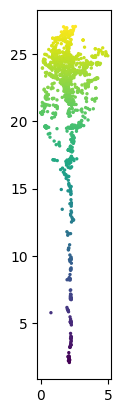
\includegraphics[width=\textwidth]{../images/03d_augmentations-fig-height-dropout-output-1.png}
}
\subcaption{\label{fig-height-dropout-1}A single aspen tree with points
colored by height.}
\end{minipage}
\begin{minipage}{0.18\linewidth}
\centering{
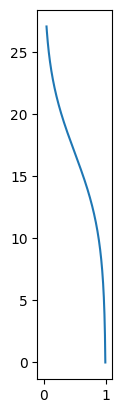
\includegraphics[width=\textwidth]{../images/03d_augmentations-fig-height-dropout-output-2.png}
}
\subcaption{\label{fig-height-dropout-2}Height-dependent probability of
dropout (a modified sigmoid).}
\end{minipage}
\begin{minipage}{0.18\linewidth}
\centering{
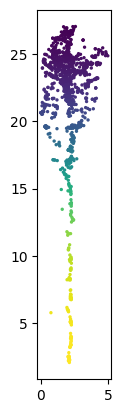
\includegraphics[width=\textwidth]{../images/03d_augmentations-fig-height-dropout-output-3.png}
}
\subcaption{\label{fig-height-dropout-3}The same aspen with points
colored by probability of dropout.}
\end{minipage}
\begin{minipage}{0.18\linewidth}
\centering{
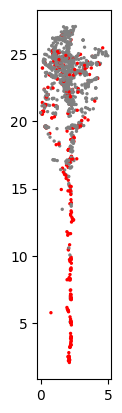
\includegraphics[width=\textwidth]{../images/03d_augmentations-fig-height-dropout-output-4.png}
}
\subcaption{\label{fig-height-dropout-4}The same aspen with points that
will be dropped marked red.}
\end{minipage}
\begin{minipage}{0.18\linewidth}
\centering{
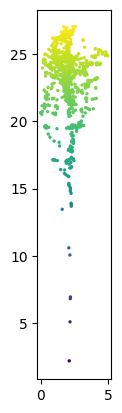
\includegraphics[width=\textwidth]{../images/03d_augmentations-fig-height-dropout-output-5.png}
}
\subcaption{\label{fig-height-dropout-5}The same aspen after the dropout
is appleid with point colored by height.}
\end{minipage}
\caption{\label{fig-height-dropout}Effect of the height-dependent
modified sigmoid dropout on a single aspen tree.}
\end{figure}

\subsubsection{Per-patch augmentations}

Random rotation within $[0; 45]$ degrees range.

\subsection{Other training parameters}

The batch size is limited by the available GPU device memory, and in the described setup competes for memory space with the synthetic forest patch dimensions used in the training dataset.
The preference is given to the size of the patch, so the batch size is set to 1, but is compensated for by using gradient accumulation steps – updates to the model parameters are made after the gradient is accumulated for a set number of iterations.
This slows down the training, but enables usage of larger batches when there is not enough memory to fit them, making the training procedure overall more stable.

Early stopping \cite{precheltAutomaticEarlyStopping1998} is set up to terminate training early if there is no improvement in average validation loss in a set number of epochs.
This makes sure that valuable GPU time is not wasted on continuing training models that are likely to have started overfitting.

The best model is saved using the accuracy as a metric.

The learning rate schedule is set to follow a fast linear warm up and slow linear decay.

Training was performed on a NVIDIA A100-SXM4-80GB GPU with X memory.
Inference works even on a much smaller GPU Tesla T4 

\subsection{On implementation of PointNet++}

As mentioned in the introduction, the PointNet++ is implemented using the PyTorch Geometric library designed for writing and training graph neural networks.
This makes the implementation not exactly the same as described in the PointNet papers.
Input transform and feature transfrom networks are not define explicitly, but local networks that process features learn to perform a similar function.
The main ideas, namely local feature learning and max pulling for permutation-invariant aggregation, are there.
Sequential application of PointNetConv layers allows the network to learn hierarchical features.

\section{Training segmented trees processing models}\label{sec-training-tree-processors}

$\lambda_1 \ge \lambda_2 \ge \lambda_3$

The features are defined as follows:

$$
\begin{aligned}
\text{linearity} &= \frac{\lambda_1 - \lambda_2}{\lambda_1} \\
\text{planarity} &= \frac{\lambda_2 - \lambda_3}{\lambda_1} \\
\text{scatter} &= \frac{\lambda_3}{\lambda_1}  \\
\text{omnivariance} &= \sqrt[3]{\lambda_1\lambda_2\lambda_3} \\
\text{anisotropy} &= \frac{\lambda_1 - \lambda_3}{\lambda_1} \\
\text{eigentropy} &= -\sum_{i=1}^{3} \lambda_i \ln(\lambda_i) \\
\text{sum of eigenvalues} &= \lambda_1 + \lambda_2 + \lambda_3 \\
\text{curvature} &= \frac{\lambda_3}{\lambda_1 + \lambda_2 + \lambda_3} \\
\end{aligned}
$$

Insert an image from IGARSS paper that visualizes the effects

\section{Matching detected trees to ground truth}

To evaluate the results, an automated and deterministic method for matching detected trees to the ground truth data is required.
It should determine which ground truth trees, if any, the detected candidates correspond to.
It should also classify all the trees from both sets as either a true positive, meaning that the ground truth tree was successfully detected, a false negative, meaning that a ground truth tree was not detected, or a false positive, meaning a tree was detected when there is none.

We implemented a matching procedure that considers the locations and heights of the trees, and falls back to using only locations when the height information is not available for the ground truth tree.
It is parametrized by the maximum allowed 2D distance and the maximum height difference between a detected and a ground truth tree to consider them a match.
First, it constructs a distance matrix between the ground truth tree locations and the detected candidates and filters out the pairs for which the distance is larger than the allowed maximum.
It then iterates over the remaining pairs in the order of increasing distance, and marks the pairs with suitable heights in which both trees are not yet assigned a class as a true positive.
The pairs in which one of the trees is already assigned a class are marked as either a false positive or a false negative, and the pairs in which both trees are assigned a class are skipped.
Finally, it marks all unmatched ground truth trees as false negatives, and all unmatched candidate trees as false positives.